\documentclass[es,practica]{uah}

\usepackage{hyperref}

\tema{A2}
\titulo{Audio sintético con LMMS}{}
%
\begin{document}

\titulacion{Grados Informática}
\asignatura{Sistemas Audiovisuales y Aplicaciones Multimedia}{}
\curso{2021/2022} 

\maketitle



En esta práctica vamos a utilizar el programa LMMS \href{https://lmms.io}{https://lmms.io}, que permite crear música sintética y mezclarla. Aunque el programa tiene multitud de opciones y permite hacer cosas bastante elaboradas, vamos a limitarnos a crear una canción muy sencilla para hacernos una idea general de su funcionamiento. Como siempre, sed libres de modificar este ejemplo a vuestro gusto, con otra canción de vuestro gusto. 

Tal y como podéis ver en el vídeo, empezad borrando las pistas que aparecen por defecto en el programa, para trabajar con un proyecto vacío. 

El primer paso va a ser crear la melodía. Para ello el primer paso es seleccionar un instrumento. Haced click en el icono con forma de estrella que hay en la barra de la izquierda. Se desplegará una lista de \emph{Mis preconfiguraciones}. Abrid la carpeta de \emph{Triple Oscillator}. Si mantenéis pulsado el botón izquierdo del ratón sobre cada uno de los instrumentos podéis escuchar una muestra del sonido. 


Coged el Xilófono (\emph{Xylophon}) y arrastradlo sobre la ventana del editor de canciones (\emph{Song editor}). Debería aparecer una nueva línea al final con el instrumento. 


Para empezar a añadir notas a esta pista, haced doble click sobre el primer cuadrado negro en la fila del xilófono, y se abrirá el editor de teclado, que podemos utilizar para ir introduciendo notas.  

Las notas que yo he introducido en el vídeo son {\bf La4, Sol4, La4, Mi4, Do4, Mi4 y La3}, reduciendo la duración de las seis primeras. En el piano aparece marcada una tecla blanca como C4 (C es Do en nomenclatura anglosajona). A partir de ahí, el resto de teclas blancas hacia arriba serían el resto de las notas: Re, Mi, Fa, Sol, La y Si. 

Por si os sirve de referencia, aquí tenéis las notas:

\begin{figure}[h!]
  \centering
  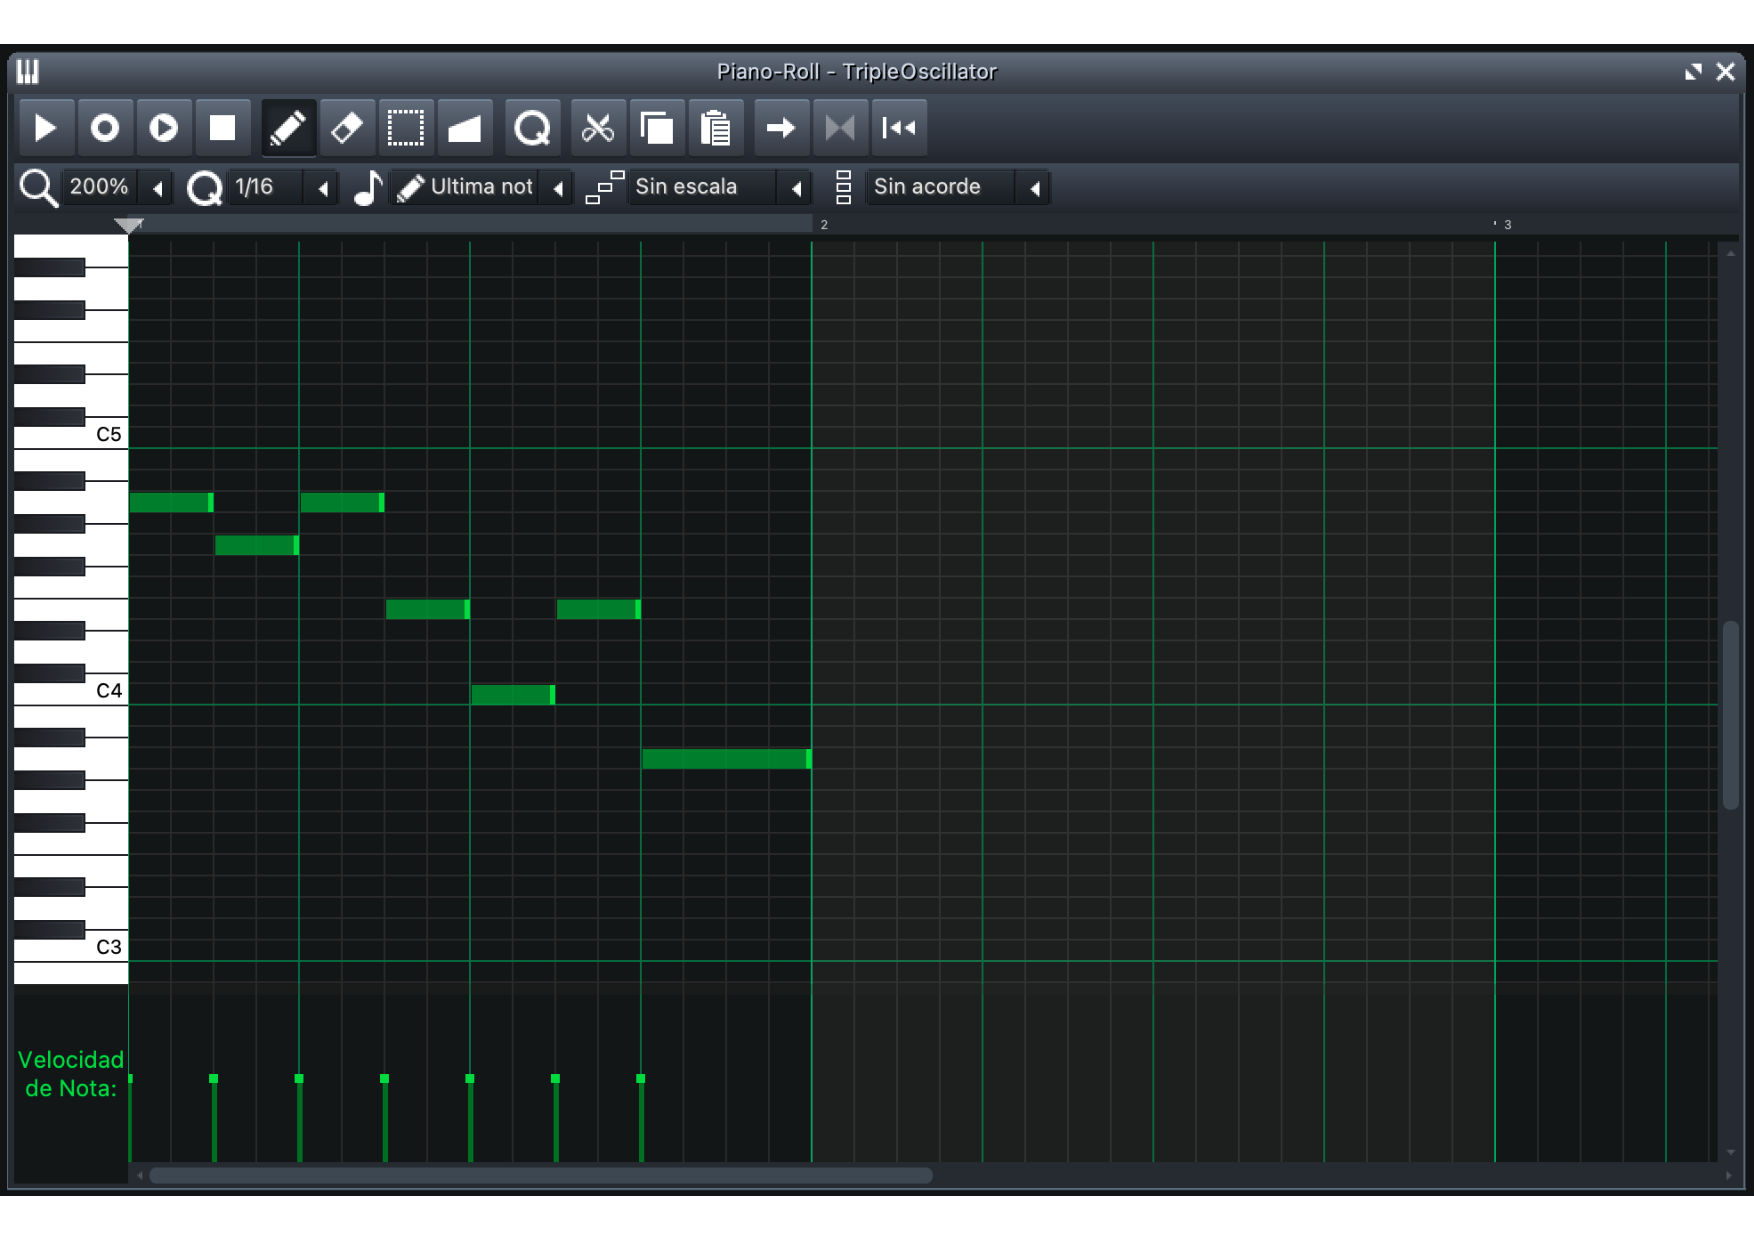
\includegraphics[width=14cm]{Figuras/Notas}
  \caption{Notas La-Sol-La-Mi-Do-Mi-La}
\end{figure}

Para repetir esta secuencia de notas hay dos formas:

\begin{itemize}
\item La más sencilla, pero también la peor, es volver a introducirlas una a una. 
\item Otra opción es utilizar la función \emph{duplicar}. Para eso, manteniendo pulsada la tecla Control (Comando en Mac), dibujad un rectángulo que permita seleccionar todas las notas. Ahora pulsad Shift y arrastrad las notas nuevas al principio del compás siguiente. 
\end{itemize}

Y ahora por último podéis completar la melodía con algunas notas más: La4, Si4, Do5, Si4, Do5, La4, Si4, La4, Si4, Sol4, La4, Sol4, La4, Fa4 y La4.

Ahora que ya tenemos la melodía, vamos a crear un ritmo de batería que la acompañe. Para ello, haced click en el icono con forma de nota musical que hay en la barra de menús de la izquierda. En la lista que se abre, seleccionad \emph{Drums}.

A partir de ahora vamos a trabajar con la ventana del editor de ritmos. En esa ventana ya aparece un bombo (\emph{Kicker}). Arrastrad también una caja (\emph{Snare}, cualquiera vale), un hihat cerrado (\emph{hihat\_closed}) y un hihat abierto (\emph{hihat\_opened}), y cread un ritmo como este (he hecho click en el botón con un + que hay arriba a la derecha para ampliar el número de compases que aparecen):

\begin{figure}[h!]
  \centering
  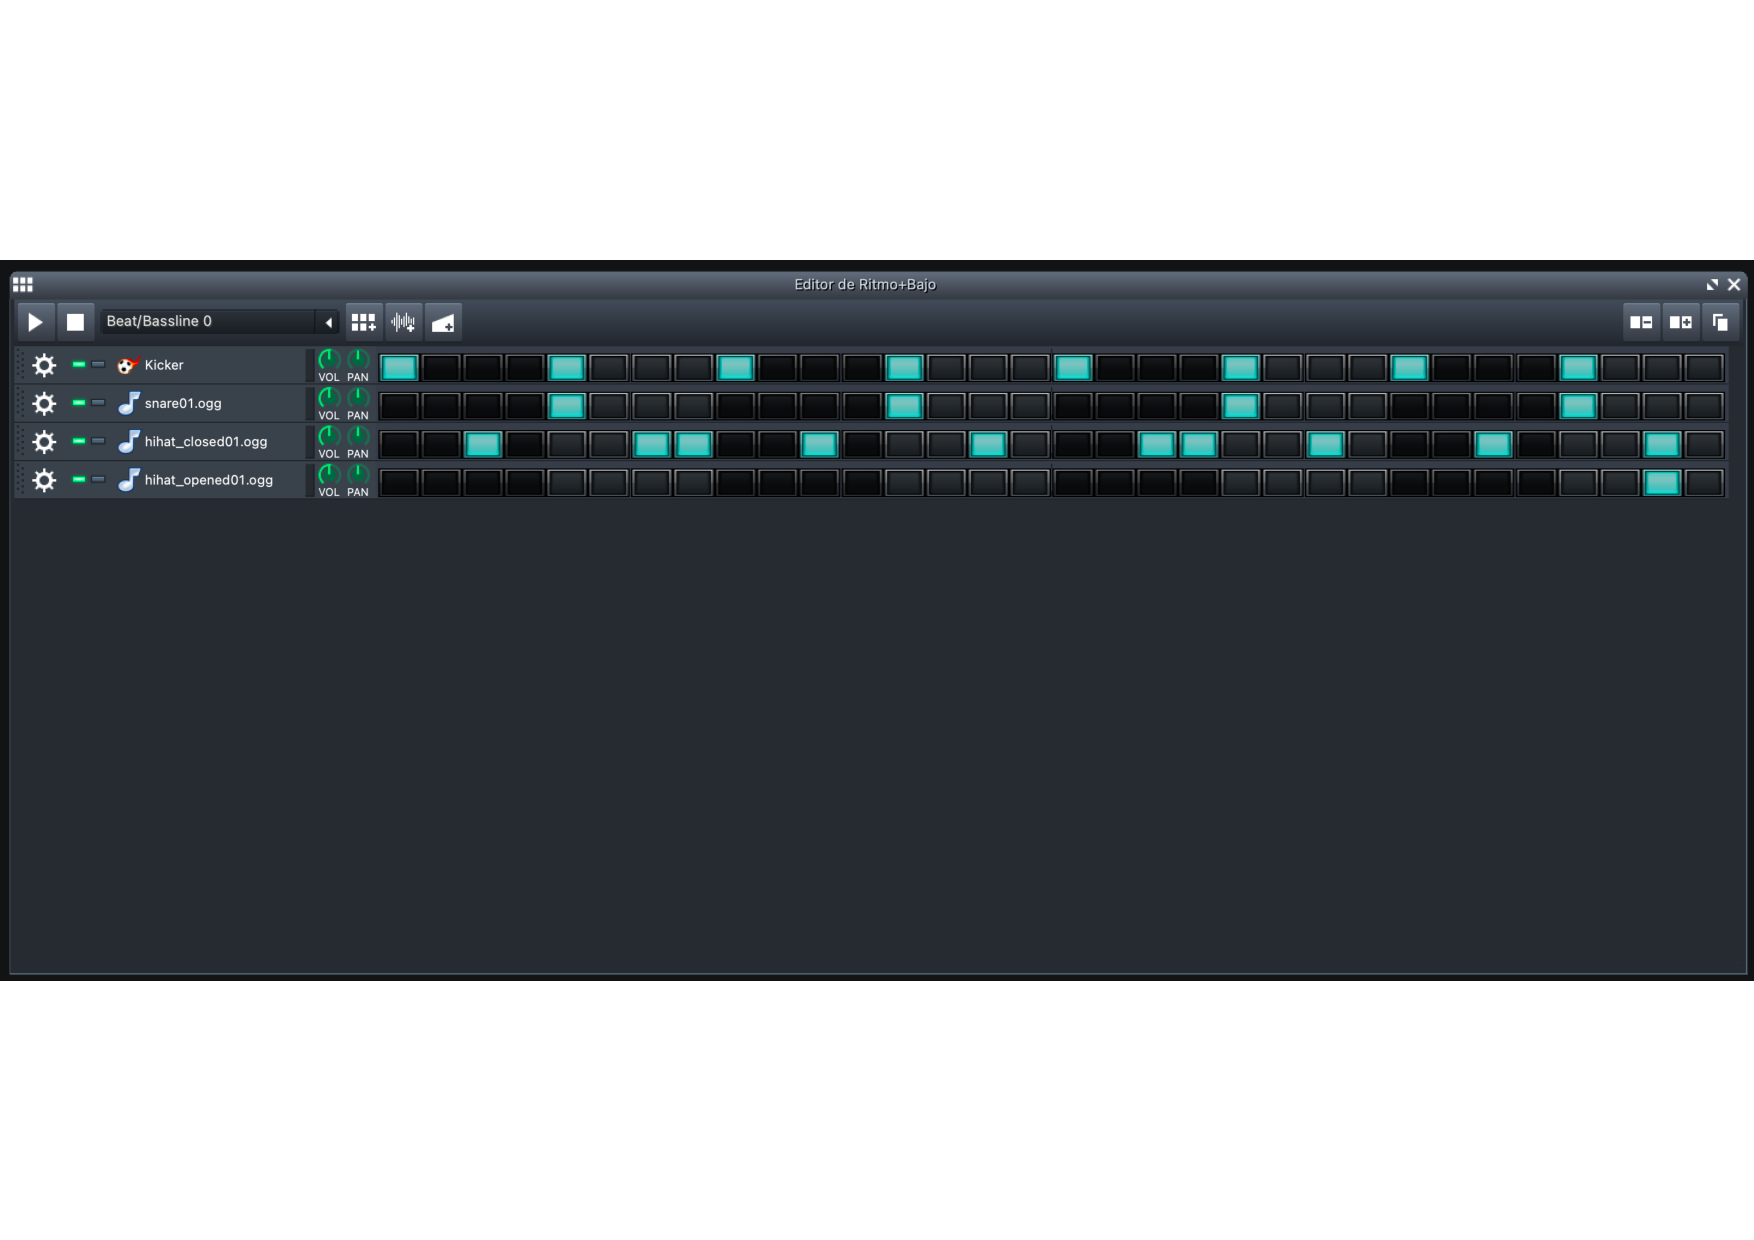
\includegraphics[width=12cm]{Figuras/Ritmo}
  \caption{Ritmo de batería creado.}
\end{figure}

Para terminar, lo único que tenemos que hacer es hacer click en el primer cuadrado dentro de la fila de la línea de ritmos en el editor de la canción, y alargar su duración para que sea igual que la del xilófono.

Ya tenemos nuestra canción de prueba terminada. Aunque con una canción tan sencilla poco se puede hacer, a partir de aquí se puede pasar al proceso de mezcla, que suele incluir, por ejemplo, los siguientes procesos:

\begin{itemize}
\item Ajustar los niveles de cada una de las pistas para asegurarse de que el sonido no llega a saturar nunca. Eso se comprueba mirando el indicador de nivel de sonido del mezclador, y asegurándose de que no está continuamente en el nivel rojo. Se puede ajustar el volumen de cada una de las pistas que tengamos de forma individual mediante el botón que pone VOL.
\item Ajustar la panorámica de cada pista. La panorámica es la posición en la que se escucha el sonido (izquierda o derecha), y se ajusta con el mando que pone PAN en cada una de las pistas.
\item Editar el sonido de cada instrumento. En nuestro ejemplo hemos utilizado un sonido preestablecido (Xilófono), pero si hacéis click sobre el nombre de la pista, se abre una nueva ventana que permite editar todos los parámetros del instrumento. Lo mismo se aplica a cada uno de los sonidos de la pista de batería.
\item Añadir efectos. Se pueden añadir efectos a cada instrumento, utilizando la pestaña FX que hay dentro de la ventana de edición del sonido del instrumento. Pulsad en \emph{Añadir efecto} y podéis seleccionar algún efecto de los disponibles. También se puede aplicar un efecto a la mezcla final añadiéndolo en la ventana del mezclador (\emph{Mezcladora FX}).
\item Añadir un instrumento nuevo. Podemos añadir un instrumento nuevo, tal y como hicimos al principio de la práctica. Para copiar las notas musicales que hemos creado de una pista a otra, o para duplicarlas en la misma pista, poned el ratón sobre la pista, y pulsando Control (o Comando en Mac), arrastradla a donde queráis que se copie. Si no, el típico copiar y pegar también funciona. 
\item Veréis también que hay una pista que se llama \emph{Automation track}. Esta pista permite definir algún tipo de automatismo para controlar algún parámetro de la mezcla. Se puede, por ejemplo, dibujar una curva que será la que siga el volumen de la pista a lo largo de la canción. Esto se utiliza por ejemplo, para hacer que el sonido de un instrumento aparezca poco a poco en la canción, o se vaya de forma gradual. 
\item También veréis que hay una pista llamada \emph{Sample track}. Este tipo de pistas se utilizan para introducir ficheros de sonido que tengamos grabados en el ordenador. Un ejemplo es cuando estamos creando una canción y tenemos grabada la pista de la guitarra tocada por nosotros. 
\end{itemize}


Recordad grabar la canción (Project - Save). Si os apetece ver ejemplos bastante más elaborados que este, en el segundo de los iconos de la barra de la izquierda (uno que tiene el símbolo del programa, una especie de cascos), tenéis varias demos. 


%
%
%
%
%
%\section{Manejo básico de una caja de ritmos - Hydrogen}
%
%Vamos a crear una canción muy simple en Hydrogen compuesta por cuatro patrones distintos, que llamaremos A, B, C y D.
%
%Cada patrón lo podemos entender como una parte de la canción: los versos, el estribillo, el puente, etc. Eso es lo que se ve en la parte superior de la ventana del Hydrogen. 
%
%Seleccionando un patrón en la parte de arriba, lo que vemos abajo son los distintos instrumentos que tenemos a nuestra disposición y una matriz de puntos en la que podemos marcar cuándo queremos que suene cada uno de ellos. 
%
%Antes de empezar, fijad la velocidad a 98bpm y la resolución a 16 (Figura \ref{fig:captura1}).
%
%\begin{figure}[h!]
%  \centering
%  \includegraphics[width=0.6\textwidth]{Captura1}
%  \caption{Configuración inicial}
%  \label{fig:captura1}
%\end{figure}
%
%Para crear un nuevo patrón, seleccionad el instrumento ``Closed HH'', haced click con el botón derecho y seleccionad ``Llena notas''. Después, insertad a mano las notas en los instrumentos ``Snare Jazz'' y ``Kick'' tal y como se muestra en la Figura \ref{fig:PatternA}. Con esto ya tenemos la base para nuestra canción. Fijaros que he modificado la intensidad de las notas del HiHat de modo que los golpes que caen al principio de cada compás tienen un valor y el resto otro inferior. Así se consigue crear un ritmo más realista. 
%
%\begin{figure}[h!]
%  \centering
%  \includegraphics[width=0.6\textwidth]{PatternA}
%  \caption{Patrón A}
%  \label{fig:PatternA}
%\end{figure}
%
%Renombrad el patrón que acabamos de crear en el editor de canciones y en lugar de ``Pattern 1'' poned, por ejemplo, ``A''. Haced ahora click con el botón derecho sobre el nombre y seleccionad ``copiar''. Ponedle a la copia el nombre ``B''. Seleccionad este nuevo patrón (importante!) y eliminad los dos últimos golpes del ``Closed HH''. Aumentad la resolución a 32 y añadid al final un par de golpes de ``Open HH'' con la intensidad como se muestra en la figura \ref{fig:PatternB}.
%
%\begin{figure}[h!]
%  \centering
%  \includegraphics[width=0.6\textwidth]{PatternB}
%  \caption{Patrón B}
%  \label{fig:PatternB}
%\end{figure}
%
%Repetid ahora el mismo proceso de antes para crear los patrones ``C'' y ``D''.
%
%\begin{figure}[h!]
%  \centering
%  \includegraphics[width=0.6\textwidth]{PatternC}
%  \caption{Patrón C}
%  \label{fig:PatternC}
%\end{figure}
%
%\begin{figure}[h!]
%  \centering
%  \includegraphics[width=0.6\textwidth]{PatternD}
%  \caption{Patrón D}
%  \label{fig:PatternD}
%\end{figure}
%
%Por último, configurad en la rejilla de arriba el orden en el que se van a reproducir los patrones que habéis creado. Ahora podéis escuchar la canción completa seleccionando la opción ``song'' en lugar de ``pattern'' arriba del todo. 
%
%\begin{figure}[h!]
%  \centering
%  \includegraphics[width=0.6\textwidth]{Patterns}
%  \caption{Sucesión de patrones}
%  \label{fig:Patterns}
%\end{figure}
%


\section{Materiales a entregar}

El archivo LMMS de la canción que hemos creado de ejemplo y, si lo habéis hecho, el archivo con cualquier otra canción con la que hayáis estado practicando.


\end{document}

	
